\section{Build Jobs}

Build jobs predstavlja skup poslova u koji spadaju kompajliranje, testiranje, pakovanje, razvijanje projekta ili bilo koji drugi posao koji manevriše sa vašim projektom. Build job je osnovni pojam kad se govori o principu kontinualne integracije. 

\subsection{Kreiranje Build Job-a}

Pravljenje build job-a je veoma jednostavno i ono podrazumeva razna podešavanja. Prvo treba odrediti kakvog će tipa biti projekat. Postoje četiri osnovne vrste i to su:
\begin{itemize}  
\item Slobodan projekat(Freestyle software project) - Vrsta projekta koji pružaju maksimalnu fleksibilnost i koji služe za osnovnu upotrebu
\item Maven project - buiild job koji je specijalno namenjen Maven projektima 
\item External job - ova opcija služi da se prate izvršavanja nekog drugog procesa koji se ne pokreće na Jenkins-u
\item Multi-configuration project - ova opcija je pogodna za projekte koji zahtevaju više različitih konfigurisanja
\item Copy existing job - projekat može da bude i kopija već postojećeg projekta koji zahteva neke promene u konfigurisanju
\end{itemize}  

\subsection{Kreiranje slobodnog projekta}

Slobodan projekat je najfleksibilnija vrsta i može se koristiti za bilo koju vrstu projekta. Puno opcija koje se nameštaju u okviru slobodnog projekta se javljaju i u ostalim vrstama projekta. Pri kreiranju projekta prvo se unose osnovni podaci kao što su ime projekta i opis projekta. Zatim slede opcije:

\begin{itemize}  
\item Discard Old Builds - čekiranjem ove opcije limitirate broj build-ova koji će se čuvati, postoje dva kriterijuma 
\begin{enumerate}
\item Po starosti - build se briše posle određenog vremena
\item Po broju - čuva se N build-ova
\end{enumerate}
\item This build is parameterized - build uzima parametre
\item Disable Build - kad je čekirano privremeno se obustavlja build-ovanje
\item Execute concurrent builds if necessary
\end{itemize}

"Napredne" opcije:
\begin{itemize}  
\item Quiet period - ako je čekirano onda sledeći zakazani build je na čekanju
\item Retry Count - u slučaju da build ne uspe, zadaje se broj ponovnih pokušaja
\item Block build when upstream project is building - sprečava se build-ovanje ako je neki projekat koji je zavistan od njega isto u procesu build-ovanja
\item Block build when downstream project is building - sprečava se build-ovanje ako je neki projekat koji je "dete" isto u procesu build-ovanja
\item Use custom workspace
\item Keep the build logs of dependencies
\end{itemize}

\subsection{Integracija sa izvornim kodom}

Jedna od najbitnijih i najznačajnijih stvari je integracija sa sistemom za kontrolu verzija. Jenkins prati svaku promenu u vašem izvornom kodu posle kojih se pokreće kompajliranje i razni automatski testovi. Podržani su razni sistemi za kontrolu verzija, CVS i Subversion "u startu", dok za sisteme kao što su Git, Mercurial, Harvest, BitKeeper i ostale postoje plugin-ovi koji se lako instaliraju preko Jenkins plugin Manager-a. Pri pravljenju projekta i odabiru koji sistem za kontrolu verzija će se koristiti, unošenjem URL-a repozitorijuma se vrši integracija sa izvornim kodom.

\subsection{Git Setup}

Da bismo mogli da se povežemo sa Git-om prvo moramo instalirati Git. Za operativne sisteme Windows i Mac OS postoje instalacije, a na Linuxu se instalira putem jednostavne komande:

\begin{verbatim}
 sudo apt-get install git-core
\end{verbatim}

Za razliku od sistema za kontrolu verzija kao što su CVS i Subversion čiji su plugin-ovi već instalirani, plugin za Git, koji se nalazi u Jenkins-ovom plugin Manager-u, morate sami instalirati. Nakon instalacije pri pravljenju novog projekta, u opcijama za biranje sistema za kontrolu verzija otvoriće se opcija i za Git što je prikazano na slici \ref{fig:git}

\begin{figure}[h!]
\begin{center}
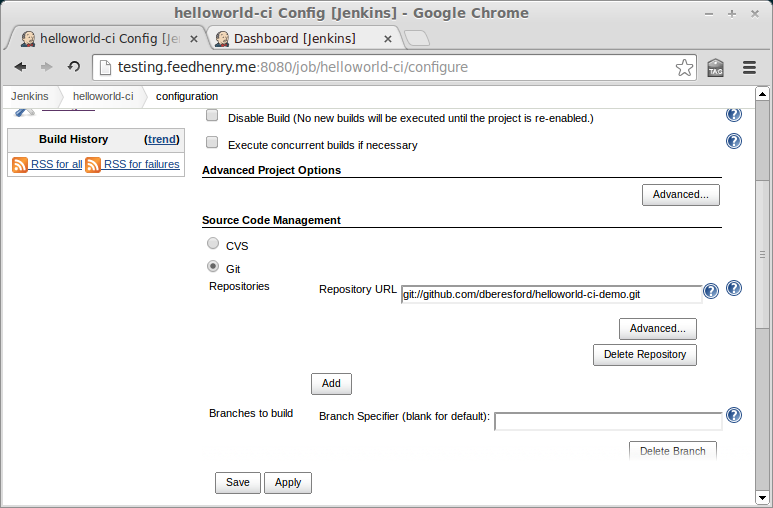
\includegraphics[scale=0.75, totalheight=0.4\textheight]{slike/git_jenkins.jpg}
\end{center}
\caption{Git}
\label{fig:git}
\end{figure}

Uz opcije "Repository" gde se navodi URL repozitorijuma i "Branches to build" gde se navodi ime branch-a(grane) koje se build-uje postoje je tzv. "Dodatna ponašanja"(Additional Behaviours). Neka od njih su:
 
\begin{itemize}  
\item Polling ignores commits from certain paths
\begin{enumerate}
\item Included regions - unose se putanje fajlova koje se build-uju
\item Excluded regions - unose se putanje fajlova čije testiranje nema efekta npr. slike
\end{enumerate}
\item Polling ignores commits in certain users 
\begin{description}
\item Excluded users - imena user-a od čije strane ne može da se pokrene build-ovanje
\end{description}
\end{itemize}

\subsection{Pokretanje build-ova}

Nakon nameštanja koji ćete sistem za kontrolu verzija koristiti, vreme je da se konfiguriše kada će se build-ovi pokretati. Postoje osnovne tri vrste pokretanja build-ova, a to su:

\begin{itemize}
  
\item Build after other projects are built
Ova opcija pruža pokretanje build-a kad god se neki drugi build izvrši. Postoje i 3 dodatne opcije:
\begin{itemize}  
\item Trigger only if build is stable - pokreni build samo ako je build stabilan
\item Trigger even if the build is unstable - pokreni build iako je build nestabilan
\item Trigger even if the build fails - pokreni build iako build ne uspe
\end{itemize}

\item Build periodically

Odlika kontinualne integracije jeste kontinualno izvršavanje build-ovanja nakon svake promene što nije stvar kod periodičnog build-ovanja. U nekim slučajevima je i pogodno koristiti ovu vrstu pokretanja npr. kod projekata gde iscrpna testiranja traju i po nekoliko sati i gde je pogodnije pokretati build-ove u određenim vremenskim intervalima.
Sintaksa za zadavanje vremenskog intervala: \\
MINUTE HOUR DOM MONTH DOW
\begin{itemize}
\item MINUTE - minut u satu (0-59)
\item HOUR - sat u danu (0-23)
\item DOM - dan u mesecu (1-31)
\item MONTH - mesec(1-12)
\item DOW - dan u nedelji(0-7) gde su 0 i 7 nedelje
\end{itemize}

\item Poll SCM

Bolja strategija od periodičnog build-ovanja jeste Polling the SCM tzv. "ispitivanje" sistema za kontrolu verzija. Ideja je da se sistem za kontrolu verzija "ispituje" da li je napravljena izmena u izvornom kodu. U slučaju da jeste Jenkins će pokrenuti build.
\end{itemize}

\subsection{Build steps}

Definisanjem build koraka govorite Jenkins-u šta da radi sa vašim izvornim kodom. Jedan build može da ima više koraka u koje spadaju izvršavanje shell skripte, izvršavanje Windows batch komande ili povezivanje sa Maven-om ili Ant-om.

\subsection{Post-Build Actions}

Nakon samog procesa build-ovanja potrebno je preduzeti neke akcije. Neke od mogućih akcija su:
\begin{itemize}
\item Archive the artifacts - ova opcija omogućava da se rezultati build-ovanja čuvaju u određenom formatu i da se zatim download-uju
\item E-mail Notifications - Jenkins obaveštava mejlom svaki put kada build ne uspe, kada uspe build nakon neuspelog pokušaja, kada je build nestabilan nakon uspešnog build-ovanja.
\end{itemize}